\subsection{Выбор и сравнение языковых моделей}
В процессе разработки диалогового агента для ролевых игр одним из ключевых решений стал выбор языковой модели, которая обеспечила бы оптимальный баланс между качеством генерации текста, быстродействием и возможностью локального запуска. Ориентация на локальные модели была продиктована следующими практическими соображениями:
\begin{itemize}
\item необходимость полного контроля над обработкой пользовательских данных;
\item отсутствие зависимости от внешних API и связанных с ними ограничений;
\item возможность тонкой настройки параметров инференса;
\item снижение эксплуатационных расходов при масштабировании проекта;
\item стабильность работы независимо от внешних сервисов.
\end{itemize}

Для разработки и тестирования использовалась видеокарта NVIDIA A100, предоставленная компанией МТС, что позволило эффективно работать с вычислительно-требовательными моделями. Рассматривались несколько высокопроизводительных моделей, способных работать на данном оборудовании: QwQ-32B, DeepSeek-R1-Distill-Qwen-32B, а также Falcon-40B \cite{reddit_a100}. Эти модели представляют собой современные языковые системы с различными архитектурными особенностями, размерами и характеристиками, что делает их сравнительный анализ важным этапом проектирования диалоговой системы для ролевых игр.
\subsubsection{Подход к выбору моделей}

При отборе языковых моделей для системы был применен многофакторный подход, учитывающий как технические возможности оборудования, так и специфические требования ролевой игры. Основные критерии оценки включали:

\begin{itemize}
\item \textbf{Качество генерации текста} — способность модели создавать связные, тематически релевантные ответы, соответствующие сеттингу древнего мира;
\item \textbf{Скорость инференса} — время отклика модели при генерации ответов, критически важное для поддержания естественного темпа диалога;
\item \textbf{Способность к поддержанию контекста} — умение модели сохранять последовательность в рамках продолжительной беседы;
\item \textbf{Понимание игровых сценариев} — корректная интерпретация запросов, связанных с военно-политическими событиями, социальными явлениями и государственным устройством;
\item \textbf{Устойчивость к нестандартным запросам} — адекватная реакция на провокационные вопросы и попытки выхода за рамки роли;
\item \textbf{Языковое разнообразие} — богатство лексики и стилистических приёмов при описании вымышленных государств, религий и культур.
\end{itemize}

Для объективного сравнения был разработан набор тестовых сценариев, моделирующих типичные ситуации в игре: создание новых государств, генерация событий (позитивных и негативных), описание культурных и религиозных особенностей. Все модели тестировались на одном и том же оборудовании (NVIDIA A100) для обеспечения сопоставимости результатов по скорости обработки запросов.
\subsubsection{Экспериментальное сравнение}

В рамках исследования было проведено сравнительное тестирование трех перспективных языковых моделей: QwQ-32B, DeepSeek-R1-Distill-Qwen-32B и Falcon-40B. Все модели были протестированы на идентичном наборе сценариев, отражающих ключевые аспекты игрового процесса в сеттинге древнего мира.

Результаты сравнения представлены в таблице, где оценки выставлялись по пятибалльной шкале:

\begin{table}[h]
\centering
\caption{Сравнительная оценка языковых моделей}
\label{tab:compare_models}
\begin{tabular}{|l|c|c|c|}
\hline
\textbf{Критерий} & \textbf{QwQ-32B} & \textbf{DeepSeek-32B} & \textbf{Falcon-40B} \\
\hline
Качество & 4 & 4.5 & 1 \\
\hline
Скорость & 3 & 5 & 2 \\
\hline
Поддержание & 3.5 & 4 & 1 \\
\hline
Понимание & 4 & 4 & 1 \\
\hline
Устойчивость & 2 & 4 & 1 \\
\hline
Разнообразие & 4 & 4 & 1 \\
\hline
Русский & \textbf{0} & \textbf{4} & \textbf{3} \\
\hline
\textbf{Сумма} & \textbf{20.5} & \textbf{29.5} & \textbf{10} \\
\hline
\end{tabular}
\end{table}


Как видно из результатов, модель DeepSeek-R1-Distill-Qwen-32B продемонстрировала наилучшие показатели по большинству критериев, особенно выделяясь по скорости инференса, качеству генерации и поддержке русского языка. Модель QwQ-32B показала хорошие результаты на английском языке, особенно в плане языкового разнообразия и понимания игровых сценариев, но практически не поддерживала русский язык, что критически важно для целевой аудитории проекта. Модель Falcon-40B показала неудовлетворительные результаты по всем параметрам, не справившись с базовыми игровыми сценариями.

Полные протоколы тестирования с примерами ответов моделей на различные запросы представлены в Приложении \ref{appendix:3}, что позволяет получить более детальное представление о качественных различиях между моделями.

\subsection{Архитектура и ключевые компоненты}
Разработанная система представляет собой комплексное программное решение, объединяющее языковую модель, асинхронные обработчики запросов и интерфейс мессенджера для создания интерактивного игрового мира. Архитектура проекта построена на принципах асинхронности, что позволяет обрабатывать запросы от множества пользователей одновременно без блокировки основного потока выполнения. Каждый компонент системы выполняет строго определённую функцию, а состояние игроков и игрового мира надёжно сохраняется в базе данных, обеспечивая персистентность и целостность игрового процесса между сессиями. Ключевая особенность реализации заключается в эффективной организации взаимодействия между пользовательским интерфейсом в Telegram, механизмом извлечения релевантной информации (RAG) и языковой моделью DeepSeek, обеспечивающей генерацию контекстно-зависимых ответов с учётом истории государства, особенностей мира и текущих игровых событий.
\subsubsection{Схема взаимодействия компонентов}

Архитектура системы построена на основе модульного подхода с чёткой сегментацией ответственности между компонентами. Общая схема взаимодействия элементов представлена на рисунке \ref{fig:flowchart}.

\begin{figure}[h]
    \centering
    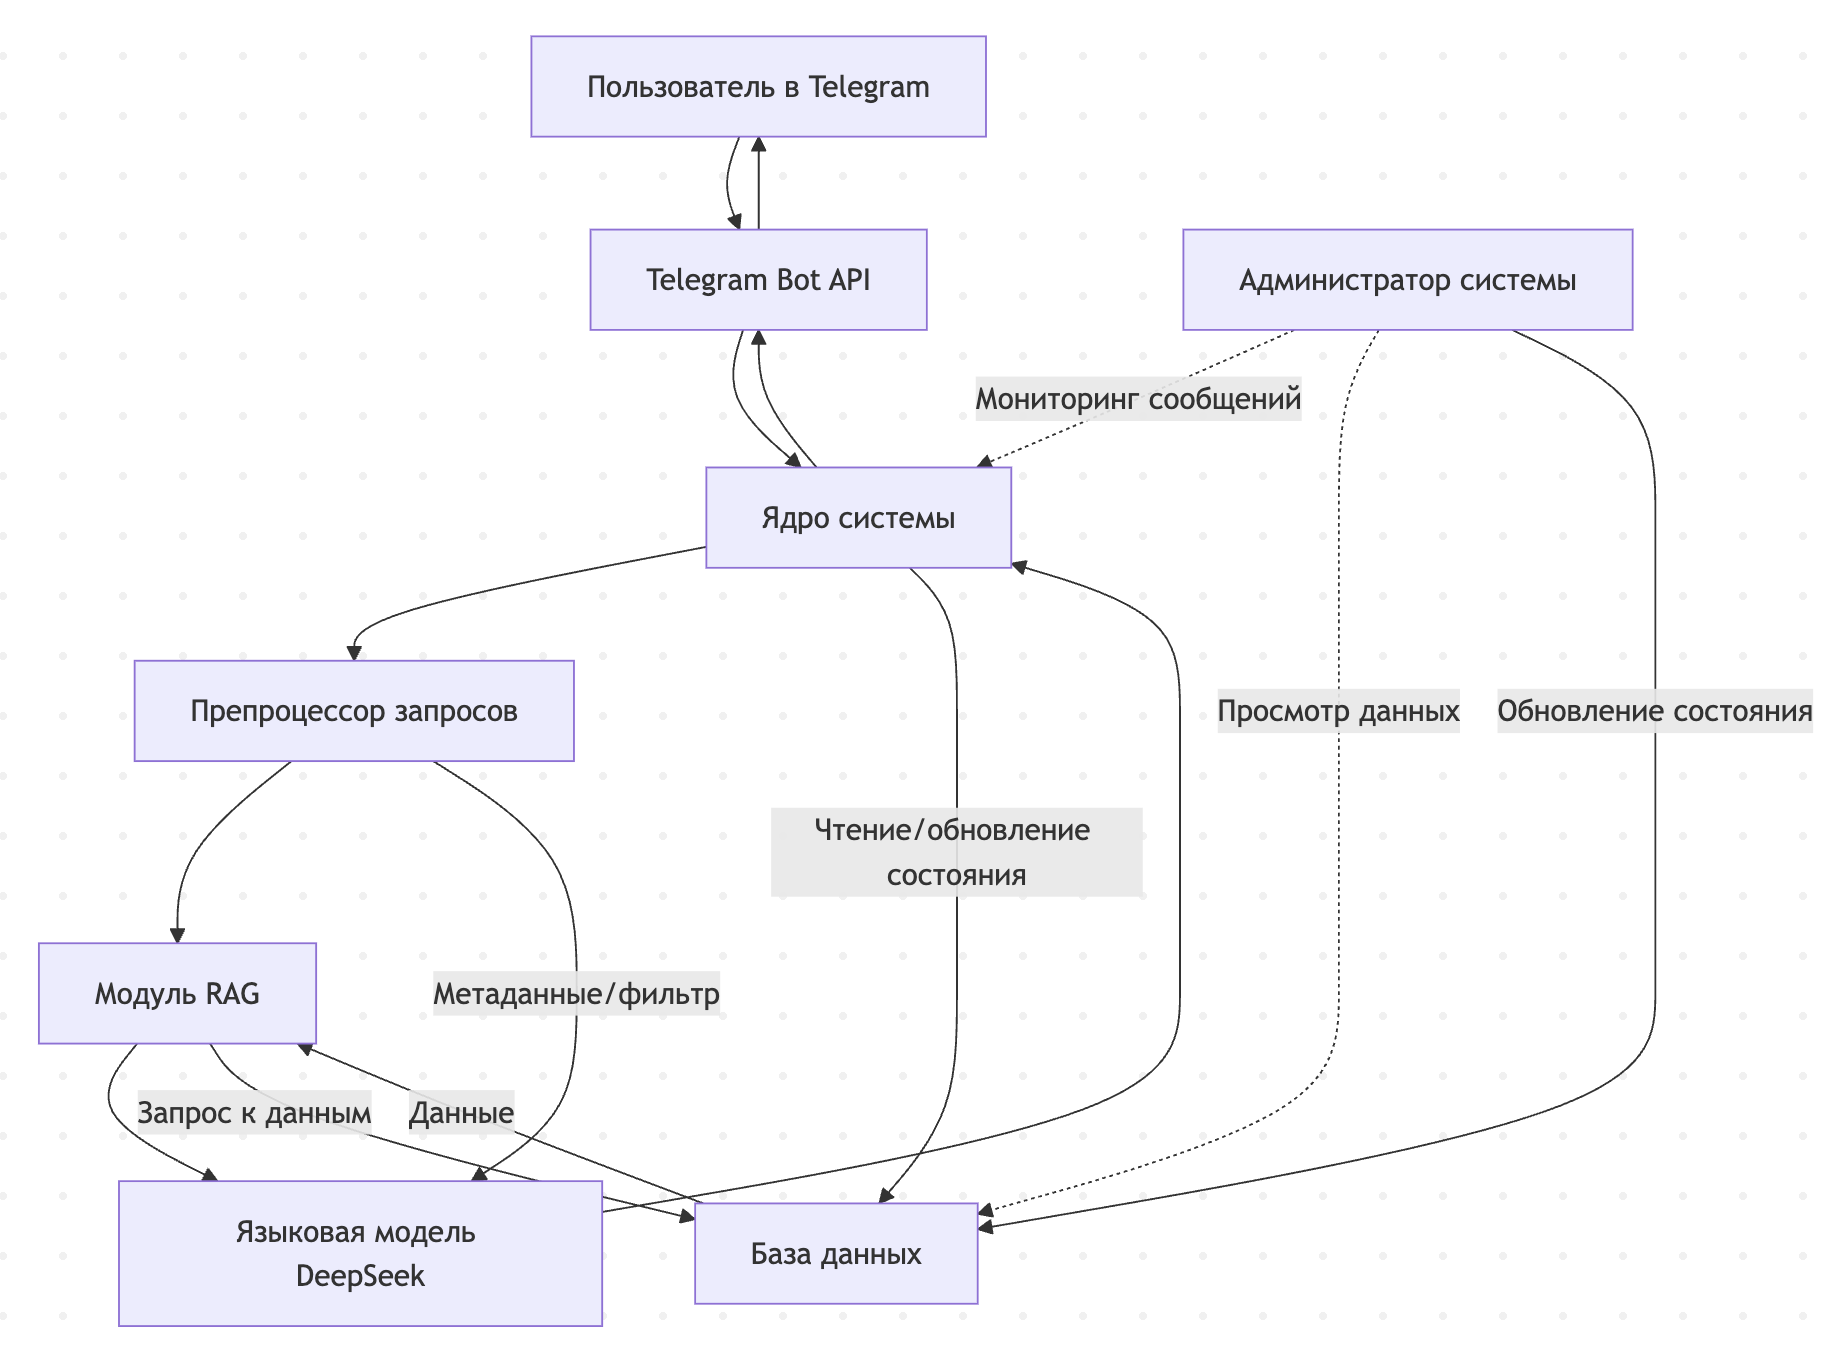
\includegraphics[width=0.8\textwidth]{figures/flowchart}
    \caption{Архитектура системы и взаимодействие компонентов}
    \label{fig:flowchart}
\end{figure}\\
~\\~\\~\\~\\~\\

Центральным звеном архитектуры выступает ядро системы, координирующее взаимодействие между всеми компонентами. Поток данных начинается с пользовательского интерфейса в Telegram, где игроки отправляют сообщения и команды. Telegram Bot API транслирует эти запросы в асинхронный обработчик сообщений, который определяет тип запроса и маршрутизирует его в соответствующий функциональный модуль.

Для обработки игровых взаимодействий задействуется цепочка компонентов:

\begin{itemize}
\item \textbf{Препроцессор запросов} анализирует входящие сообщения, фильтрует запрещенные термины и подготавливает контекст для языковой модели.

\item \textbf{Модуль RAG (Retrieval-Augmented Generation)} извлекает из базы данных релевантную информацию об игровом мире, стране игрока и исторических событиях, обогащая контекст запроса.

\item \textbf{Языковая модель DeepSeek} генерирует ответы на основе обогащенного контекста, сохраняя согласованность с игровым миром и стилистическую уместность.

\item \textbf{База данных} хранит информацию о пользователях, странах, игровых событиях и истории взаимодействий, обеспечивая персистентность игрового мира.
\end{itemize}

Асинхронная природа системы позволяет обрабатывать запросы от множества игроков одновременно, не блокируя основной поток выполнения. Каждый запрос обрабатывается в отдельной задаче, что оптимизирует использование ресурсов и повышает отзывчивость системы.

Для администраторов реализован отдельный интерфейс управления, позволяющий мониторить состояние системы, вносить коррективы в игровой мир и разрешать возникающие конфликтные ситуации без прерывания игрового процесса для остальных пользователей.

\subsubsection{Подсистема управления контекстом}

В текущей версии системы реализована базовая подсистема управления контекстом, основанная на принципах RAG (Retrieval-Augmented Generation). Данная подсистема выполняет две ключевые функции: обогащение запросов релевантной информацией и фильтрацию анахронизмов.

Механизм обогащения контекста работает через сопоставление ключевых слов в запросе пользователя с предопределенными категориями игрового мира. Например, если в сообщении игрока обнаруживаются слова, связанные с экономической тематикой (такие как "экономик", "торгов", "богатств", "финанс", "ресурс", "бюджет", "деньги", "доход", "налог"), система автоматически извлекает из базы данных релевантную информацию об экономике государства пользователя и добавляет её в контекст запроса к языковой модели.

Аналогичным образом функционирует и система фильтрации анахронизмов. Предварительно составленный словарь современных терминов и понятий (например, "интернет", "смартфон", "ядерное оружие", "демократия", "конституция") используется для проверки сообщений пользователя на соответствие историческому антуражу. При обнаружении таких слов система предупреждает пользователя о нарушении стилистики игрового мира и предлагает переформулировать запрос.

В текущей реализации используется относительно простой подход на основе ключевых слов, однако система спроектирована с учетом возможности последующей интеграции более сложных семантических алгоритмов и векторных представлений для повышения точности извлечения релевантной информации и определения контекста запросов.

\subsubsection{Механизмы обработки запросов пользователя}

Обработка пользовательских запросов в системе представляет собой многоэтапный процесс, обеспечивающий релевантность, историческую достоверность и стилистическое соответствие генерируемых ответов:

\begin{enumerate}
\item \textbf{Предварительная фильтрация:} Каждый запрос пользователя анализируется на наличие современных терминов и анахронизмов. В случае обнаружения слов, не соответствующих историческому сеттингу (например, "танк", "радио", "демократия"), система предупреждает пользователя о нарушении стилистических рамок и запрашивает переформулировку сообщения.

css
\item \textbf{Контекстное обогащение:} На основе семантического анализа запроса определяются тематические категории, к которым он относится (экономика, военное дело, религия и т.д.). Затем система автоматически извлекает из базы данных релевантную информацию об этих аспектах как для государства пользователя, так и для других стран, с которыми возможно взаимодействие. Эта информация включается в промпт для языковой модели.

\item \textbf{Формирование системного промпта:} К пользовательскому запросу добавляется системный промпт, определяющий роль и ограничения для языковой модели. Он включает инструкции по стилю ответа, ограничения на использование современных концепций и указания по соблюдению исторического антуража.

\item \textbf{Генерация ответа:} Обогащенный запрос передается в локальную языковую модель DeepSeek, которая генерирует ответ на основе предоставленной информации и контекста.

\item \textbf{Постпроцессинг:} Сгенерированный ответ подвергается дополнительной обработке. Удаляются служебные теги (например, \texttt{<think>...</think>}), которые модель могла использовать для "{}рассуждений"{}, отсекаются потенциально нерелевантные части ответа.
\end{enumerate}

Благодаря этому многоступенчатому процессу система обеспечивает согласованность игрового мира, предотвращает использование анахронизмов и поддерживает высокий уровень вовлеченности игроков через контекстно-зависимые, исторически достоверные ответы.

\subsubsection{Регистрация и учёт игроков}

Процесс регистрации в игровой системе реализован максимально просто, требуя от пользователя минимальных усилий и одновременно обеспечивая полноценное вхождение в игровой мир. При первом взаимодействии с ботом пользователю предлагается создать собственное государство в сеттинге древнего мира. Для этого необходимо указать лишь два базовых параметра: название страны и краткое описание её ключевых особенностей.

На основе предоставленной пользователем информации языковая модель автоматически генерирует расширенное описание государства, включающее следующие аспекты:
\begin{itemize}
\item \textbf{Экономика:} клады, дары, источники богатств и торговые пути, кои питают казну державы
\item \textbf{Военное дело:} войско, число ратников, устроение и крепости, что хранят границы державы
\item \textbf{Внешняя политика:} дела междержавные, сношения с соседями, союзы и старые вражды
\item \textbf{Территория:} земли подвластные, их пределы, реки, горы, леса и иные природные дары
\item \textbf{Технологичность:} мудрость ремесленников, кузнецов, зодчих и иные достижения мастерства
\item \textbf{Религия и культура:} боги и верования, коим благоговейно поклоняются жители страны
\item \textbf{Управление и право:} власть государя, уставы, древние законы и порядок в суде да совете
\item \textbf{Строительство и инфраструктура:} дворцы, стены, ристалища, гавани, мосты и иные великие строения державы
\item \textbf{Общественные отношения:} сословия, нравы народа, старейшины и положения в чинах и кланах
\end{itemize}

Стоит отметить, что набор аспектов является гибким и может быть настроен администратором системы в соответствии с конкретными игровыми потребностями или спецификой моделируемого исторического периода.

Вся сгенерированная информация структурируется и сохраняется в базе данных SQLite, что обеспечивает быстрый доступ к ней в дальнейшем процессе игры. Такой подход позволяет не только упростить процесс вхождения нового игрока в игру, но и гарантирует, что все аспекты созданного государства будут гармонично вписываться в общий сеттинг и соответствовать исходной задумке пользователя.

\subsubsection{Интеграция с Telegram}

Реализация интерфейсного слоя системы через платформу Telegram обеспечивает доступность игры широкому кругу пользователей и предоставляет ряд преимуществ с точки зрения пользовательского опыта. Для улучшения интерактивности взаимодействия были интегрированы специальные механизмы Telegram API.

В частности, при обработке запроса пользователя и генерации ответа языковой моделью (что может занимать несколько секунд) система автоматически отправляет сигнал ``печатает...'' через метод \texttt{messages.setTyping} \cite{telegram_typing}. Это создаёт у пользователя интуитивно понятное ощущение живого диалога и даёт понять, что бот активно работает над ответом, а не просто игнорирует запрос.

Для администрирования игрового процесса был создан специальный групповой чат, доступный только для ведущих игры. В этом чате реализован расширенный набор команд, позволяющих:
\begin{itemize}
\item просматривать полную информацию о любом государстве
\item редактировать отдельные аспекты государств игроков
\item создавать и рассылать глобальные игровые события
\item вносить изменения в базу данных с помощью упрощённого синтаксиса команд
\item отслеживать активность пользователей и статистику использования системы
\end{itemize}

Такая архитектура администрирования обеспечивает оперативное управление игровым процессом без необходимости прямого доступа к серверу или базе данных, что значительно упрощает поддержку и модерацию игры.

\subsection{Проверка соответствия ответов бота требованиям}
\subsubsection{Критерии качества игровых ответов и ролевого поведения}
\subsubsection{Тестирование на антураж и отсутствие современных терминов}
\subsubsection{Типовые диалоги и анализ релевантности}
\subsubsection{Системы фильтрации и самоконтроля}

\subsection{Обратная связь и оценки пользователей}
\subsubsection{Организация раннего тестирования}
\subsubsection{Описание отзывов тестовых игроков}
\subsubsection{Изменения в системе по результатам обратной связи}

\subsection{Результаты и итоговая спецификация}
\subsubsection{Функциональные возможности финальной версии}
\subsubsection{Ограничения и известные проблемы}
\subsubsection{Перспективы дальнейшего развития}